% !TEX root = widefieldscan.tex
\svnidlong
{$HeadURL$}
{$LastChangedDate$}
{$LastChangedRevision$}
{$LastChangedBy$}
%
\section{Materials and Methods}\label{sec:materials and methods}
\subsection{Sample Preparation}
Rat lung samples, prepared according to \citeasnoun{Tschanz2002} and \citeasnoun{Luyet2002} were used as test objects. Briefly, lungs of Sprague-Dawley rats were filled with \SI{2.5}{\percent} glutaraldehyde (\cf{CH2(CH2CHO)2}) in \SI{0.03}{\Molar} potassium-phosphate buffer (pH 7.4) by instillation via tracheotomy at a constant pressure of \SI{20}{\centi\meter} water column. In order to prevent recoiling of the lung, this pressure was maintained during glutaraldehyde-fixation for a minimum of two hours. Subsequently, the lungs were dissected free and immersed in toto in the same fixative at a temperature of \SI{4}{\celsius} for at least \SI{24}{\hour}.

The samples were postfixed with \SI{1}{\percent} osmium tetroxide (\cf{OsO4}) and stained with \SI{4}{\percent} uranyl nitrate (\cf{UO2(NO3)2}) to increase the x-ray absorption contrast, dehydrated in a graded series of ethanol and embedded in paraffin using Histoclear (Merck KGaA, Darmstadt, Germany) as an intermedium. The lung samples were mounted onto standard scanning electron microscopy sample holders (PLANO GmbH, Wetzlar, Germany) using paraffin~\cite{Tsuda2008}.

The handling of animals before and during the experiments, as well as the experiments themselves, were approved and supervised by the Swiss Agency for the Environment, Forests and Landscape and the Veterinary Service of the Canton of Bern, Switzerland.

\subsection{Synchrotron radiation tomographic microscopy}
The experiments were performed at the TOMCAT beamline at the Swiss Light Source, Paul Scherrer Institut, Villigen, Switzerland. The samples were scanned at \SI{12.6}{\kilo\electronvolt}. After penetration through the sample, the x-rays were converted into visible light by a YAG:Ce scintillator (\SI{18}{\micro\meter} thickness, Crismatec Saint-Gobain, Nemours, France). Projections were magnified by diffraction limited microscope optics (10$\times$ magnification) and digitized by a high-resolution 2048$\times$2048 pixel CCD camera (pco.2000, PCO AG, Kelheim, Germany) with 14 bit dynamic range. The detector was operated in 2$\times$2 binning mode. As a result, the pixel size was \SI{1.48}{\micro\meter} and the exposure time was \SI{175}{\milli\second}.

Projections $I_{Pr}$ were recorded at equiangular positions between \SI{0}{\degree} and \SI{180}{\degree}. The exact number of angular projections depended on the selected scan protocol, as described in section~\ref{subsec:increasing the field of view}. Additionally, for each protocol a set of dark ($I_{D}$) and flat images ($I_{F}$) were recorded for noise and baseline correction, respectively. Further details of the imaging and reconstruction workflow at the TOMCAT beamline can be found in~\cite{Hintermueller2010}.

\subsection{Increasing the field of view}\label{subsec:increasing the field of view}
For parallel beam geometry, tomographic images are obtained at equidistant angles over a sample rotation of \SI{180}{\degree} as shown in Figure~\ref{fig:scanning-possibilities}(a). After reconstruction, the width of the image corresponds to the field of view of the camera.

Samples twice as large as the field of view can be imaged using scanning protocols based on a \SI{360}{\degree} off center sample rotation as shown in Figure~\ref{fig:scanning-possibilities}(b). Images recorded between \SI{180}{\degree} and \SI{360}{\degree} have to be flipped after acquisition: the projections obtained at angular position $\theta$ and $\theta$+\SI{180}{\degree} ($I_{Pr_{\theta}}$ and $I_{Pr_{\theta+\SI{180}{\degree}}}$) have to be stitched to one projection. The resulting images cover twice the field of view of the camera.

\begin{figure}
	\centering
	\caption{Covering the field of view of differently sized samples with one \SI{180}{\degree} scan (a), one \SI{360}{\degree} scan (b) or---in the case of the so called wide field scanning---with multiple subscans (three subscans, c). The filled segments mark the region of the sample that is covered while scanning the respective positions (Position 1: magenta/checkerboard, Position 2: yellow, Position 3: cyan/striped).}
\begin{tikzpicture}
	%%%%%%%%%%%%%%%%%%%
	%       180       %
	%%%%%%%%%%%%%%%%%%%
		\def\startAtY{9}
		\def\BeamLength{4}
		\def\length{2}
		\node [anchor=north] at (0.25,\startAtY) {(a)};
		%camera
			\draw [fill=gray] (0,\startAtY) rectangle (1,\startAtY+1);
			\node [anchor=center] at (0.5,\startAtY+1+.25) {camera};
		% beam
			% inner rays
			\foreach \x in {9,9.1,...,10} draw[gray!50,<-] (1,\x) -- (\BeamLength+1,\x);
			% outer rays
			\foreach \x in {0,1} \draw[<-] (1,\startAtY+\x) -- (\BeamLength+1,\startAtY+\x);
			% label				
			\node at (\BeamLength+0.5,\startAtY+1+.25) {beam};
		%sample
			\fill [color=gray, nearly transparent] (0.5*\BeamLength+1,\startAtY+0.5) circle (0.5);
			\fill (0.5*\BeamLength+1,\startAtY+0.5) circle (0.025);
			\draw [thick] (0.5*\BeamLength+1,\startAtY+0.5) circle (0.5);
			\draw [thick,->] (0.5*\BeamLength+1,\startAtY+0.25) arc (-90:90:0.25);
			\node at (0.5*\BeamLength+1,\startAtY+1+0.25) {sample};
	%%%%%%%%%%%%%%%%%%%
	%       360       %
	%%%%%%%%%%%%%%%%%%%
		\def\startAtY{6}
		\node [anchor=north] at (0.25,\startAtY) {(b)};
		%camera
			\draw [fill=gray] (0,\startAtY) rectangle (1,\startAtY+1);
		% beam
			% inner rays
			\foreach \x in {6,6.1,...,7}
				\draw[gray!50,<-] (1,\x) -- (\BeamLength+1,\x);
			% outer rays
			\foreach \x in {0,1}
				\draw[<-] (1,\startAtY+\x) -- (\BeamLength+1,\startAtY+\x);
			% label				
		%sample
			\fill [color=gray, nearly transparent] (0.5*\BeamLength+1,\startAtY+1) circle (1);
			\fill (0.5*\BeamLength+1,\startAtY+1) circle (0.025);
			\draw [thick] (0.5*\BeamLength+1,\startAtY+1) circle (1);
			\draw [thick,->] (0.5*\BeamLength+1,\startAtY+0.75) arc (-85:265:0.25);
	%%%%%%%%%%%%%%%%%%%
	% Wide Field Scan %
	%%%%%%%%%%%%%%%%%%%
		\def\startAtY{2}
		\node [anchor=north] at (0.25,\startAtY-1.5) {(c)};
		%camera
			\draw [fill=gray] (0,\startAtY) rectangle (1,\startAtY+1);
		% beam
			% inner rays
			\foreach \x in {2,2.1,...,3}
				\draw[gray!50,<-] (1,\x) -- (\BeamLength+1,\x);
			% outer rays
			\foreach \x in {0,1}
				\draw[<-] (1,\startAtY+\x) -- (\BeamLength+1,\startAtY+\x);
		% shaded samples
		\foreach \y/\position/\color in {\startAtY-0.5/1/magenta,\startAtY+0.5/2/yellow,\startAtY+1.5/3/cyan}
			{
				\fill [color=\color, nearly transparent] (0.5*\BeamLength+1,\y) circle (1.5);
			}
		%Pattern Fills in Circles
			% Position1
				\fill [color=magenta, semitransparent] (0.5*\BeamLength+1,3) arc (90:-90:1.5) -- ++(0,1) arc (-90:90:0.5);
				\fill [pattern=checkerboard, semitransparent, pattern color=gray] (0.5*\BeamLength+1,3) arc (90:-90:1.5) -- ++(0,1) arc (-90:90:0.5);
			% Position 3
				\fill [color=cyan, semitransparent] (0.5*\BeamLength+1,3+2) arc (90:270:1.5) -- ++(0,1) arc (270:90:0.5);
				\fill [pattern=horizontal lines, semitransparent, pattern color=gray] (0.5*\BeamLength+1,3+2) arc (90:270:1.5) -- ++(0,1) arc (270:90:0.5);
			% Position 2
				\fill [color=yellow, nearly opaque] (0.5*\BeamLength+1,3-0.5) circle (0.5);
		% Labels
		\foreach \y/\position/\color/\pattern in {\startAtY-0.5/1/magenta/checkerboard,\startAtY+0.5/2/yellow/,\startAtY+1.5/3/cyan/horizontal lines}
			{
				\draw[thick] (0.5*\BeamLength+1,\y) circle (1.5) circle (0.5);
				\draw[thick,->] (0.5*\BeamLength+1,\y-0.25) arc (-90:90:0.25);
				\node [fill=\color,semitransparent] at (\BeamLength+2+.005,\y-.005) {Position \position};
				\node [fill=\color,pattern=\pattern,semitransparent, pattern color=gray] at (\BeamLength+2+.005,\y-.005) {Position \position};
				\node at (\BeamLength+2+.01,\y-.01) {Position \position};
				\node [color=white] at (\BeamLength+2,\y) {Position \position};
				\fill (0.5*\BeamLength+1,\y) circle (0.025);
			}
	\end{tikzpicture}
	\label{fig:scanning-possibilities}
\end{figure}

For tomographic scans covering a size wider than two fields of view, three or more \SI{180}{\degree}-scans taken at slightly overlapping positions are combined, as shown in Figure~\ref{fig:scanning-possibilities}(c). The projections of each subscan overlap slightly to facilitate the stitching of multiple projections into a single one. The cutline, i.\,e. the position where the merging takes place, is automatically determined according to a mean squared difference method~\cite{Hintermueller2010}.

A straightforward acquisition scheme would record an equal amount of projections for each of the individual subscans. As a consequence, to fulfill the sampling theorem in the lateral parts of the sample, oversampling the central parts of the sample would be necessary.

Since the total acquisition time per sample linearly scales with the total amount of recorded projections such an acquisition scheme obviously increases the total amount of beamtime for one sample without relevantly increasing the quality of the reconstructed tomographic data. Hence, such an oversampling is generally avoided.

Our goal was to find a good compromise between scanning time and image quality. We therefore devised an acquisition scheme for covering a wide field of view based on the assumption that a sufficient resolution and contrast can be achieved in the tomographic dataset, if the sampling theorem is individually fulfilled for each of the subscans. This results in a set of $i$ subscans with $P_{i}$ projections each. A simple example with $P_{2}=4$ and $P_{1}=P_{3}=8$ is shown in Figure~\ref{fig:projections}(a). Since each subscan $i$ has a different number of projections $P_{i}$, the stitching algorithm has to interpolate missing projections from adjacent projections (represented by the dotted lines in Figure~\ref{fig:projections}(b)) to generate a complete set of merged projections for reconstruction.

As a by-product, such an optimization of the individual number of projections $P_{i}$ for each subscan $i$ decreases the total acquisition time for one sample and thus the imparted radiation dose.

\begin{figure}
	\centering
	\caption{Wide field scan setup with three \SI{180}{\degree} scans; one central (yellow) and two lateral scans (magenta and cyan or top and bottom, respectively). In this drawing, four projections for the central and eight projections for each of the lateral scans have been recorded. The colors of the three positions correspond to the colors shown in Figure~\ref{fig:scanning-possibilities}(c). %
	(a): scanned projections %
	(b): scanned projections and additional interpolated projections (dotted) required to merge all projections.}
	\def\radius{1}%
	\def\gap{0.05}%
	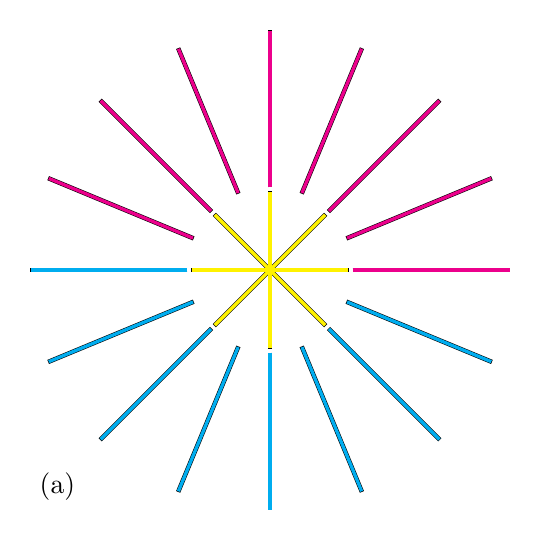
\begin{tikzpicture}
		\foreach \ang in {0,45,...,359}%
			{%
			\draw [ultra thick] (\ang:0) -- (\ang:\radius);%
			}%
		\foreach \ang in {0,45,...,359}%
			{%
			\draw [very thick, color=yellow, shorten >=0.25pt] (\ang:0) -- (\ang:\radius);%
			}%
		\foreach \ang in {0,22.5,...,179}%
			{%
			\draw [ultra thick] (\ang:\radius+\gap) -- (\ang:3*\radius+\gap);%
			\draw [very thick, color=magenta, shorten >=0.25pt,shorten <=0.25pt] (\ang:\radius+\gap) -- (\ang:3*\radius+\gap);%
			}%
		\foreach \ang in {180,202.5,...,359}%
			{%
			\draw [ultra thick] (\ang:\radius+\gap) -- (\ang:3*\radius+\gap);%		
			\draw [very thick, color=cyan, shorten >=0.25pt,shorten <=0.25pt] (\ang:\radius+\gap) -- (\ang:3*\radius+\gap);%
			}%
		\node [anchor=south west] at (-3.05,-3.05) {(a)};
	\end{tikzpicture}
	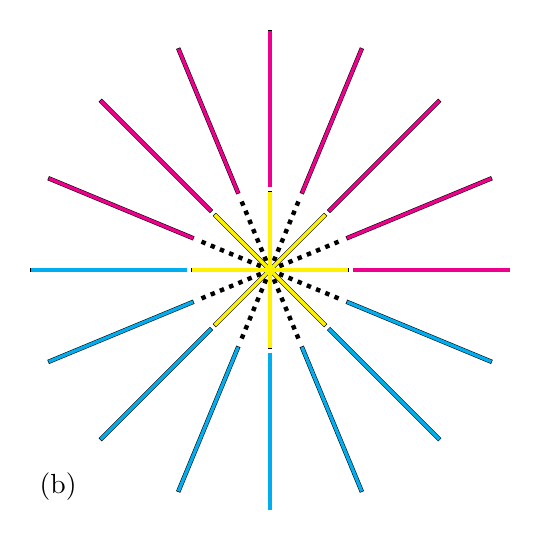
\begin{tikzpicture}
		\foreach \ang in {22.5,67.5,...,359}%
			{%
			\draw [ultra thick, dotted] (\ang:0) -- (\ang:\radius);%
			}%
		\foreach \ang in {0,45,...,359}%
			{%
			\draw [ultra thick] (\ang:0) -- (\ang:\radius);%
			}%
		\foreach \ang in {0,45,...,359}%
			{%
			\draw [very thick, color=yellow, shorten >=0.25pt] (\ang:0) -- (\ang:\radius);%
			}%
		\foreach \ang in {0,22.5,...,179}%
			{%
			\draw [ultra thick] (\ang:\radius+\gap) -- (\ang:3*\radius+\gap);%		
			\draw [very thick, color=magenta, shorten >=0.25pt,shorten <=0.25pt] (\ang:\radius+\gap) -- (\ang:3*\radius+\gap);%
			}%
		\foreach \ang in {180,202.5,...,359}%
			{%
			\draw [ultra thick] (\ang:\radius+\gap) -- (\ang:3*\radius+\gap);%
			\draw [very thick, color=cyan, shorten >=0.25pt,shorten <=0.25pt] (\ang:\radius+\gap) -- (\ang:3*\radius+\gap);%
			}%
		\node [anchor=south west] at (-3.05,-3.05) {(b)};
	\end{tikzpicture}
	\label{fig:projections}
\end{figure}	

We defined a gold standard protocol and several additional scanning protocols in order to compare different acquisition schemes. The gold standard protocol covers the desired field of view while fulfilling the sampling theorem---which states that for a detector width of $D$ pixels, we need to acquire a number of projections $P=D\frac{\pi}{2}$~\cite{Kak2002}---in all its regions, as shown in Figure~\ref{fig:SubScan-Setup}(a). In this case we need to achieve a field of view of 3072 pixels. The dark gray circle is the field of view that could be covered using a large detector with a size of 3072 pixels and recording $P=3072\frac{\pi}{2}=4825$ projections.

Using a detector with a size of 1024 pixels, this desired field of view could be covered with nine independent local tomography scans. Such an approach would require nine independent reconstructions and stitching of those nine reconstructed tomographic datasets into one dataset covering the full field of view. This method would also introduce artifacts at the edges of each of the nine sub-datasets which would lie inside the sample to be imaged.

While the chosen field of view of 3072$\times$3072 pixels can be covered using a detector of the size of 3072 pixels in one scan, we can cover the desired field of view with a much smaller detector, using a scanning protocol with three subscans from which we obtain merged projections. Figure~\ref{fig:SubScan-Setup}(b) shows how the desired field of view of 3072 pixels can be covered with a wide field scan, composed of one central and two half ring-scans, recorded with a small detector with a size of 1024 pixels and 4825 projections per subscan (a total of 14475 projections) which are then subsequently merged to 4825 large projections spanning the whole field of view. A further increase in the field of view can be obtained by simple iteration. Figures~\ref{fig:SubScan-Setup}(c)--(f) show such a setup for a five- or seven-fold increase.

\begin{figure}
	\centering
	\caption{Setup for different field of views. %
		(a): Desired field of view of 3072 pixel diameter. %
		(b): Wide field scanning protocol for covering the desired field of view of panel (a) with merged projections from one central and two half ring scans ($r_{1}$ and $r_{2}$). %
		(c): Desired field of view of 5120 pixel diameter. %
		(d): Wide field scanning protocol for covering the desired field of view of panel (c) with merged projections from one central and four half ring scans ($r_{1}$--$r_{4}$). %
		(e): Desired field of view of 7168 pixel diameter. %
		(f): Wide field scanning protocol for covering the desired field of view of panel (e) with merged projections from one central and six half ring scans ($r_{1}$--$r_{6}$).}%
	\def\width{2.75}
	\def\size{3}%
	\def\angle{150}
	\def\scale{\width/\size}
	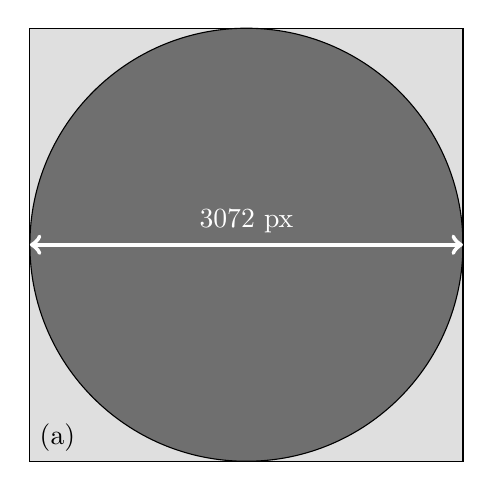
\begin{tikzpicture}[scale=\scale]
		%\draw [dashed] (-1,-1) grid (7,7);
		\draw [fill=gray!25] (0,0) rectangle (2*\size,2*\size);
		\fill [semitransparent] (\size,\size) circle (\size);
		\draw (\size,\size) circle (\size);
		\draw [white, ultra thick,<->] (0,\size) -- node [above] {3072 px} (2*\size,\size);
		\node [anchor=south west] at (0,0) {(a)};%
	\end{tikzpicture}%
	%	\hfill%
	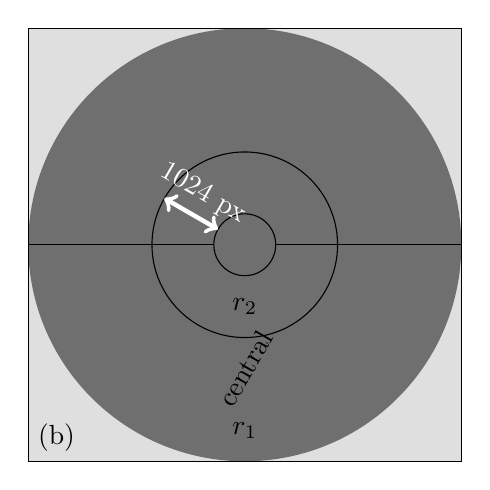
\begin{tikzpicture}[scale=\scale]
		%\draw [dashed] (-1,-1) grid (7,7);
		\draw [fill=gray!25] (0,0) rectangle (2*\size,2*\size);
		\fill [semitransparent] (\size,\size) circle (\size);
		\foreach \r in {1,3} \draw (\size,\size) circle (\r);
		\draw (0,\size) -- (\size-1,\size);
		\draw (\size+1,\size) -- (2*\size,\size);
		\node at (\size,1) {$r_{1}$};
		\node [rotate=270+\angle] at (\size,3) {central};
		\node at (\size,5) {$r_{2}$};
		\draw [white, ultra thick,<->] (\size,\size) +(\angle:1) -- node [sloped,midway,above] {1024 px} +(\angle:3); 
		\node [anchor=south west] at (0,0) {(b)};%
	\end{tikzpicture}%
	%%%%%%%%%%%%%%%%%%%%%%%%%%%%% 3 SUBSCANS
	%%%%%%%%%%%%%%%%%%%%%%%%%%%%% 5 SUBSCANS
	\def\size{5}%
	\def\scale{\width/\size}
	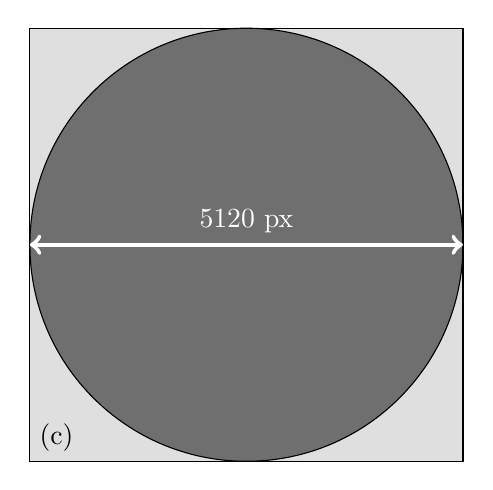
\begin{tikzpicture}[scale=\scale]%
		%\draw [dashed] (-1,-1) grid (7,7);
		\draw [fill=gray!25] (0,0) rectangle (2*\size,2*\size);
		\fill [semitransparent] (\size,\size) circle (\size);
		\draw (\size,\size) circle (\size);
		\draw [white, ultra thick,<->] (0,\size) -- node [above] {5120 px} (2*\size,\size);
		\node [anchor=south west] at (0,0) {(c)};%
	\end{tikzpicture}%
	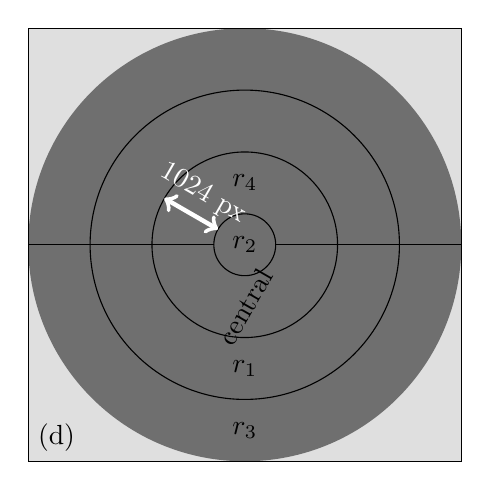
\begin{tikzpicture}[scale=\scale]
		%\draw [dashed] (-1,-1) grid (7,7);
		\draw [fill=gray!25] (0,0) rectangle (2*\size,2*\size);
		\fill [semitransparent] (\size,\size) circle (\size);
		\foreach \r in {1,3,5} \draw (\size,\size) circle (\r);
		\draw (0,\size) -- (\size-1,\size);
		\draw (\size+1,\size) -- (2*\size,\size);
		\node at (\size,1) {$r_{3}$};
		\node at (\size,3) {$r_{1}$};
		\node [rotate=270+\angle] at (\size,5) {central};
		\node at (\size,7) {$r_{2}$};
		\node at (\size,9) {$r_{4}$};
		\draw [white, ultra thick,<->] (\size,\size) +(\angle:1) -- node [sloped,midway,above] {1024 px} +(\angle:3); 
		\node [anchor=south west] at (0,0) {(d)};%
	\end{tikzpicture}%
	%%%%%%%%%%%%%%%%%%%%%%%%%%%%% 5 SUBSCANS
	%%%%%%%%%%%%%%%%%%%%%%%%%%%%% 7 SUBSCANS
	\def\size{7}%
	\def\scale{\width/\size}
	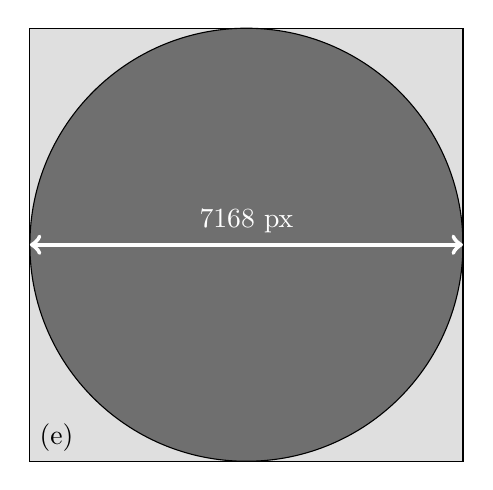
\begin{tikzpicture}[scale=\scale]%
		%\draw [dashed] (-1,-1) grid (7,7);
		\draw [fill=gray!25] (0,0) rectangle (2*\size,2*\size);
		\fill [semitransparent] (\size,\size) circle (\size);
		\draw (\size,\size) circle (\size);
		\draw [white, ultra thick,<->] (0,\size) -- node [above] {7168 px} (2*\size,\size);
		\node [anchor=south west] at (0,0) {(e)};%
	\end{tikzpicture}%
	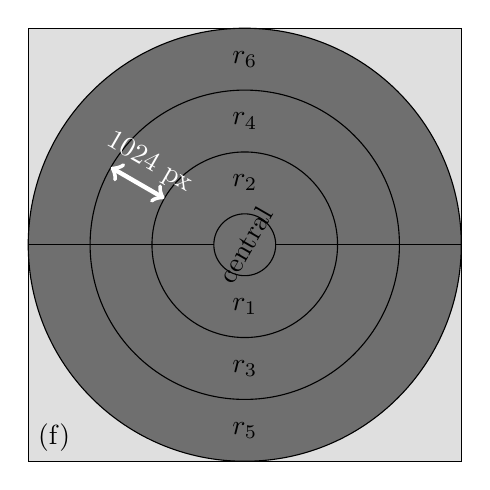
\begin{tikzpicture}[scale=\scale]
		%\draw [dashed] (-1,-1) grid (7,7);
		\draw [fill=gray!25] (0,0) rectangle (2*\size,2*\size);
		\fill [semitransparent] (\size,\size) circle (\size);
		\foreach \r in {1,3,5,7} \draw (\size,\size) circle (\r);
		\draw (0,\size) -- (\size-1,\size);
		\draw (\size+1,\size) -- (2*\size,\size);
		\node at (\size,1) {$r_{5}$};
		\node at (\size,3) {$r_{3}$};
		\node at (\size,5) {$r_{1}$};
		\node [rotate=270+\angle] at (\size,7) {central};
		\node at (\size,9) {$r_{2}$};
		\node at (\size,11) {$r_{4}$};
		\node at (\size,13) {$r_{6}$};
		\draw [white, ultra thick,<->] (\size,\size) + (\angle:3) -- node [sloped,midway,above] {1024 px} +(\angle:5);
		\node [anchor=south west] at (0,0) {(f)};%
	\end{tikzpicture}%
	\label{fig:SubScan-Setup}
\end{figure}

\subsection{Quality guided protocols}\label{sec:quality guided protocols}
Taking the experimental constraints like desired field of view, available detector size, magnification and binning into account, a MATLAB-script calculates a set of acquisition protocols. Each such protocol contains the number of projections for each subscan linearly scaled in total amount of projections from a gold standard scan down to a protocol where the sampling theorem is far from being satisfied (Table~\ref{tab:protocols}). Through optimization of the number of recorded projections, a reduction of the total acquisition time by \SI{84}{\percent} (compared to the gold standard) was achieved.

Using a Shepp-Logan phantom~\cite{Shepp1974} with added Gaussian noise as a reference image, a simulated tomographic scan and subsequent reconstruction was calculated for each of these acquisition protocols. For each protocol we calculated the expected reconstruction quality using the difference image between the reconstruction of this protocol and the initial reference image. This simulated reconstruction quality was plotted against the total acquisition time (red dots in Figure~\ref{fig:NormalizedErrorPlot}).

The end-user---balancing between acquisition time and desired image quality---chooses one protocol from the presented set for scanning his sample. A file containing all the details of the chosen scan is written to disk, and parsed by a custom Python-script. This script interacts with the hardware control system at the TOMCAT beamline enabling an automated, unattended batch acquisition of all necessary subscans.

To assess the simulations in a real world example, we selected nineteen different acquisition protocols with varying number of projections to scan one single sample (details are specified in Table~\ref{tab:protocols}, including the calculated Quality for each protocol).

A scan covering the chosen field of view with nine independent local tomography scans, each with a field of view of 1024$\times$1024 pixels, would need a total of $P=9(1024\frac{\pi}{2})=14476$ projections. This protocol was not considered for this study, since the sampling theorem can be equally satisfied by acquiring the required amount of projections with one central and two ring scans, as defined in section~\ref{subsec:increasing the field of view}. Including an overlap of 100 pixels between the central and the ring scan, an equivalent wide field scanning protocol (Protocol A in Table~\ref{tab:protocols}) requires the acquisition of 13534 projections ($P_{A}=3(3072-200)\frac{\pi}{2}$).

Protocols B--T have been linearly scaled down with a decreasing number of acquired projections of the ring scans. To simplify interpolation and merging of the projections from each subscan, we only selected acquisition schemes where the number of projections of the inner and the outer subscans is the same or a multiple of two (see figure~\ref{fig:projections}). This constraint also led to a slight oversampling for protocol B, otherwise the number of projections for each subscan of this protocol ($5244=3\cdot874$) would not have scaled down nicely to the 874 projections used for protocol T.

All parameters of each protocol and each subscan (sample-position in relation to the beam, rotation angles and number of projections) were set in a preference-file, generated using aforementioned MATLAB-script. One rat lung sample was scanned using each of the 19 different protocols (B--T), without manual intervention, permitting a direct comparison of the reconstructed datasets.

\begin{table}
	\caption{Details of the 19 scanned protocols for this study (B--T): An unoptimized scan to cover the desired field of view of 3072 pixels with nine independent scans (with a detector width of 1024 pixels) would require to record a total of $P_{\textrm{Gold standard}}=9(1024)\frac{\pi}{2}=14476$ projections. The wide field scanning protocol (A) equivalent to this field of view only uses three subscans, resulting in a total number of projections of $P_{A} = 3(3072-200)\frac{\pi}{2}= 13534$. Three-dimensional reconstructions of the datasets marked with a light gray background are shown in Figure~\ref{fig:BvsT}.}
	\label{tab:protocols}
	\begin{tabular}{ccccccc}
		\multirow{2}{*}{Protocol} & \multicolumn{3}{c}{Projections for Subscan} & Total Number & Time/Radiation & Simulated\\
			& $\textrm{s}_{1}$ & $\textrm{s}_{2}$ & $\textrm{s}_{3}$        & of Projections & Dose [\%] & Quality [\%]\\
		\hline
		A\footnote{Wide field scan equivalent to an unoptimized scan covering the field of view with nine independent scans.} & & & & 13534 & 100 & \\
		\rowcolor{lightgray} B\footnote{Gold Standard for this study} & 5244 & 5244 & 5244 & 15732 & 116 & 100\\
		C & 5244 & 2622 & 5244 & 13110 &  97 & 89\\
		D & 4370 & 4370 & 4370 & 13110 &  97 & 85\\
		E & 4370 & 2185 & 4370 & 10925 &  81 & 87\\
		F & 3934 & 3934 & 3934 & 11802 &  87 & 80\\
		G & 3934 & 1967 & 3934 & 9835  &  73 & 84\\
		H & 3496 & 3496 & 3496 & 10488 &  77 & 78\\
		I & 3496 & 1748 & 3496 & 8740  &  65 & 80\\
		J & 3060 & 3060 & 3060 & 9180  &  68 & 76\\
		K & 3060 & 1530 & 3060 & 7650  &  57 & 75\\
		\rowcolor{lightgray} L  & 2622 & 2622 & 2622 & 7866  &  58 & 72\\
		M & 2622 & 1311 & 2622 & 6555  &  48 & 69\\
		N & 2186 & 2186 & 2186 & 6558  &  48 & 67\\
		O & 2185 & 1093 & 2185 & 5463  &  40 & 62\\
		P & 1748 & 1748 & 1748 & 5244  &  39 & 61\\
		Q & 1748 & 874  & 1748 & 4370  &  32 & 55\\
		R & 1312 & 1312 & 1312 & 3936  &  29 & 46\\
		S & 874  & 874  & 874  & 2622  &  19 & 21\\
		\rowcolor{lightgray} T & 874  & 437  & 874  & 2185  &  16  & 20\\
	\end{tabular}
\end{table}

\subsection{Projection merging and tomographic reconstruction}
After acquisition of the three subscans per protocol, custom MATLAB functions read the parameters of the single subscans (e.\,g. sample name, amount of subscans, amount of dark and flat images) as well as the desired output-name and -suffix, and performed all necessary calculations, including: loading of the correct projections from each subscan; normalizing; interpolation; cutline detection; correct stitching of the images into wide field projections, and writing these merged projections as well as log files needed for the reconstruction to disk.

The merged projections were subsequently rearranged into sinograms, where the $n$\textsuperscript{th} sinogram is composed of the $n$\textsuperscript{th} line of every corrected projection. The $n$\textsuperscript{th} slice of the tomographic scan was reconstructed from the $n$\textsuperscript{th} sinogram using an FFT-based regridding algorithm~\cite{Dowd1999,Marone2008}. The 19 tomographic datasets were reconstructed on a computing cluster composed of five \SI{64}{\bit} Opteron machines with four cores and \SI{8}{\giga\byte} RAM each. The reconstructions resulted in an image stack covering a large sample volume of 2792$\times$2792$\times$1024 pixels, a nine-fold increase from the standard volume of 1024$\times$1024$\times$1024 pixels for one conventional scan.